\documentclass{ximera}

\input{../preamble.tex}

\title{1.6 - Polynomial End Behavior and Graphs}
\begin{document}

\begin{abstract} \end{abstract}
\maketitle


\section{End behavior of polynomial functions}
We will shortly turn our attention to graphs of polynomial functions, but we have one more topic to discuss \emph{End Behavior}.
Basically, we want to know what happens to our function as our input variable $x$ gets really, really large in either the positive or negative direction.
This is kind of like the limits we talked about before, except $x$ is not approaching a fixed value $a$, but just going off to either the right or the left.

We'll start with the most basic polynomials, the \emph{monomials}, $x^n$.  (Since \emph{mono-} means one, the monomials are the polynomials with a single term.)
Here are the graphs of $f(x)=x^n$ for $n = 2$, $4$, and $6$:
	\begin{center}
		\begin{tikzpicture}
        			\begin{axis}[
          			domain=-2:2,
          			xmin=-2, xmax=2,
          			ymin=-8, ymax=8,
          			width=4in,
          			axis lines =middle, xlabel=$x$, ylabel=$y$,
          			every axis y label/.style={at=(current axis.above origin),anchor=south},
          			every axis x label/.style={at=(current axis.right of origin),anchor=west},
          			]
	 	 		\addplot [very thick, penColor, smooth] {x^2};
				\addplot [very thick, penColor2, smooth] {x^4};
				\addplot [very thick, penColor4, smooth] {x^6};
        			\end{axis}
      		\end{tikzpicture}
	\end{center}

	
Here are the graphs of $f(x)=x^n$ for $n = 3$, $5$, and $7$:
	\begin{center}
		\begin{tikzpicture}
        			\begin{axis}[
          			domain=-2:2,
          			xmin=-2, xmax=2,
          			ymin=-8, ymax=8,
          			width=4in,
          			axis lines =middle, xlabel=$x$, ylabel=$y$,
          			every axis y label/.style={at=(current axis.above origin),anchor=south},
          			every axis x label/.style={at=(current axis.right of origin),anchor=west},
          			]
	 	 		\addplot [very thick, penColor, smooth] {x^3};
				\addplot [very thick, penColor2, smooth] {x^5};
				\addplot [very thick, penColor4, smooth] {x^7};
        			\end{axis}
      		\end{tikzpicture}
	\end{center}

Notice the similarity between the all the graphs with $n$ even.  They all have the same basic cup shape, but higher values of $n$ make the graphs flatter in $(-1,1)$ and steeper outside $(-1,1)$.

The same thing happens with the $n$ odd graphs.  They have the same basic shape, but higher values of $n$ make the graphs flatter near the origin and steeper past $1$ and $-1$.

When $n$ is even, what is happening to the output values of $f(x) = x^n$ as $x$ gets larger and larger?  They themselves get larger and larger!  As $x$ increases without bound, so do the outputs.
The same thing happens as $x$ gets larger and larger in the negative direction without bound.  This is the end behavior we were looking for.  We'll say it this way:

\begin{align*}
	\text{As} \quad x \to \infty \, ,  \quad & x^n \to \infty \\
	\text{As} \quad x \to -\infty \, , \quad & x^n \to \infty \quad \text{, for $n$ even}
\end{align*}

For $n$ odd we have a slightly different end behavior.
\begin{align*}
	\text{As} \quad x \to \infty \, ,  \quad & x^n \to \infty \\
	\text{As} \quad x \to -\infty \, , \quad & x^n \to -\infty \quad \text{, for $n$ odd}
\end{align*}

Next we need to see how a coefficient could change this.  Remember how multiplying by a constant transforms a graph?  If the constant is positive the graph is vertically stretched/compressed.
If the constant is negative the graph is flipped over the $x$-axis and then vertically stretched/compressed.  This means if the coefficient of $x^n$ is positive, the end behavior is unaffected.  If the 
coefficient is negative, the end behavior is negated as well.

\begin{example}
	Find the end behavior of $f(x) = -3x^4$.
	\begin{explanation}
		Since $4$ is even, the function $x^4$ has end behavior 
		\begin{align*}
			\text{As} \quad x \to \infty \, ,  \quad & x^4 \to \infty \\
			\text{As} \quad x \to -\infty \, , \quad & x^4 \to \infty 
		\end{align*}
		The coefficient is negative, changing our end behavior to
		\begin{align*}
			\text{As} \quad x \to \infty \, ,  \quad & -3x^4 \to -\infty \\
			\text{As} \quad x \to -\infty \, , \quad & -3x^4 \to -\infty 
		\end{align*}
	\end{explanation}
\end{example}

\begin{problem}
	Find the end behavior of $g(x) = -6 x^9$.
	\begin{align*}
		\text{As} \quad x \to \infty \, ,  \quad & -6x^9 \to \answer{-\infty} \\
		\text{As} \quad x \to -\infty \, , \quad & -6x^9 \to \answer{\infty} 
	\end{align*}
\end{problem}


We understand monomials.  What about more general polynomials? 
\begin{example}
	Find the end behavior of $f(x) = 3x^5 - 4x^3 + 1$.
	\begin{explanation}
		If we rewrite the function as:
		\begin{align*}
			f(x) &= 3x^5 - 4x^3 + 1 \\
				&= x^5 \left( \frac{3x^5}{x^5} - \frac{4x^3}{x^5} + \frac{1}{x^5} \right)\\
				&=x^5 \left( \frac{3x^5}{x^5} - \frac{4x^3}{x^5} + \frac{1}{x^5} \right)\\
				&= x^5 \left( 3 - \frac{4}{x^2} + \frac{1}{x^5} \right)
		\end{align*}
		Remember that as $x\to \pm\infty$ we saw that $x^2 \to \infty$ and that $x^5 \to \mp \infty$.  That means $\frac{4}{x^2} \to 0$ and $\frac{1}{x^5} \to 0$. 
		(We'll talk about this more when we talk about Rational Functions.)  This means everything in parentheses will basically be just $3$ as $x \to \pm \infty$.
		That is, the polynomial $3x^5 - 4x^3 + 1$ has the same end behavior as $3x^5$.  Thus
		\begin{align*}
			\text{As} \quad x \to \infty \, ,  \quad & f(x) \to \infty \\
			\text{As} \quad x \to -\infty \, , \quad & f(x) \to -\infty 
		\end{align*}
	\end{explanation}
\end{example}

This example showed us that \emph{the end behavior of a polynomial is the same as the end behavior of its leading term}.
\begin{problem}
	Find the end behavior of $g(x) = -6x^9 + 15x^5 + 7 x^4 - 18 x^3 + 91x^2 - 72 x + 4$
	\begin{align*}
		\text{As} \quad x \to \infty \, ,  \quad & g(x) \to \answer{-\infty} \\
		\text{As} \quad x \to -\infty \, , \quad & g(x) \to \answer{\infty} 
	\end{align*}
\end{problem}


\section{What do the graphs look like?}
We understand the graphs of polynomials of degrees $1$ and $2$ very well.

Polynomial functions with degree $1$ are referred to as linear polynomials.  This is due to the fact
that such a function can be written as $f(x) = mx + b$.  The graph of such a function is a straight line
with slope $m$ and $y$-intercept at $(0,b)$.

Quadratic functions, written as $f(x) = ax^2 + bx + c$ with $a \ne 0$, have parabolas as their graphs.
\begin{example}
	Sketch the graph of the function $f(x) = \frac{1}{2} x^2 + 2x + 1$.
	\begin{explanation}
		To plot the parabola, we first complete the square to write our function in the form $f(x) = a(x-h)^2 +k$.
		\begin{align*}
			f(x) &= \frac{1}{2} x^2 + 2x + 1 \\
				&= \frac{1}{2} \left( x^2+ 4x \right) + 1\\
				&= \frac{1}{2}\left( x^2 + 4x + 4\right) + 1 - \frac{1}{2} \cdot 4\\
				&= \frac{1}{2} \left( x+2 \right)^2 -1
		\end{align*} 
		The parabola we are looking for has vertex at $(-2, -1)$, opens upward (since $1/2 > 0$), and is wider than the standard
		$y=x^2$ parabola.
		\begin{tikzpicture}
        			\begin{axis}[
          			domain=-6:2,
          			xmin=-6, xmax=2,
          			ymin=-2, ymax=8,
          			width=2.5in,
          			axis lines =middle, xlabel=$x$, ylabel=$y$,
          			every axis y label/.style={at=(current axis.above origin),anchor=south},
          			every axis x label/.style={at=(current axis.right of origin),anchor=west},
          			]
	 	 		\addplot [very thick, penColor, smooth] {0.5*x^2+2*x+1};
        			\end{axis}
      		\end{tikzpicture}
		
		In terms of graph transformations, we can think of this as the graph of $g(x) = x^2$, which has been shifted horizontally $2$ units to the left,
		vertically compressed by a factor of $\frac{1}{2}$, then shifted vertically $1$ unit downward.
	\end{explanation}
\end{example}


%\begin{problem}
%	Use the graph of $f(x) = 2x^2 - 4x + 3$ to estimate the value of $\lim_{x\to 2} f(x)$.
%	\[ \begin{prompt} 
%		\lim_{x\to 2} f(x) = \answer{3} 
%	\end{prompt}\]
%\end{problem} 

For polynomials of higher degree, we will have to take everything else we have been talking about and put it together.  
We need to understand the zeroes of the polynomial and its end behavior.  The zeroes will correspond to $x$-intercepts, and the
end behavior will tell us what happens out past those intercepts.

One upshot of the Fundamental Theorem of Algebra (in terms of graphing) is that when we plot a
polynomial of degree $n$, its graph will cross the $x$-axis \emph{at most}
$n$ times.  Each crossing corresponds to a real root of that polynomial.  (Complex roots do not give crossings!)

\begin{example}
	Sketch a rough graph of the function $f(x) = 2(x-1)^2(x+2)$.

	\begin{explanation}
		We start with the end behavior of this function.  It is a degree $3$ polynomial with leading coefficient $2$, so
		\begin{align*}
			\text{As} \quad x \to \infty \, ,  \quad & f(x) \to \infty \\
			\text{As} \quad x \to -\infty \, , \quad & f(x) \to -\infty 
		\end{align*}
		We also see from the factorization that $x=1$ is a zero of multiplicity $2$, and $x=-2$ is a zero of multiplicity $1$.
		That means our graph will have $x$-intercepts at those locations.
		
		At these $x$-intercepts, will the graph pass through the $x$-axis like a line does, or will it touch the axis and turn back
		around, like a parabola does at it's vertex?  To answer this, look at a sign-chart for $f$.

		\begin{center}
		\begin{tikzpicture} 
			\tkzTabInit[lgt=2,espcl=1] 
				{$x$         /1, 
				$2$   /1, 
				$\left(x-1\right)^2$  /1,
				$x+2$       /1}% 
				{  , $-2$ , $1$ ,  }% 
			\tkzTabLine{ , + , t , + , t , + , }
			\tkzTabLine{ , + , t , + , t , + ,}
			\tkzTabLine{ , - , t , + , t , + ,  }
		\end{tikzpicture} 
		\end{center}
		
		Notice that around $x=-2$, only the $x+2$ factor changes signs.  That means $f(x)$ will change signs, so the graph will pass through the $x$-axis at $x=-2$.
		At $x=1$, however, the $(x-1)^2$ factor does NOT change signs (due to the even exponent).  That means $f(x)$ will turn around at that $x$-intercept.  Putting
		this together, we have the following graph.
		
		\begin{center}
		\begin{tikzpicture}
        			\begin{axis}[
          			domain=-3:3,
          			xmin=-3, xmax=3,
          			ymin=-2, ymax=9,
          			width=3in,
          			axis lines =middle, xlabel=$x$, ylabel=$y$,
          			every axis y label/.style={at=(current axis.above origin),anchor=south},
          			every axis x label/.style={at=(current axis.right of origin),anchor=west},
          			]
	 	 		\addplot [very thick, penColor, smooth] {2*((x-1)^2)*(x+2)};
        			\end{axis}
      		\end{tikzpicture}
		\end{center}
	\end{explanation}
\end{example}

\begin{problem}
	The function $f(x) = -4x^4 - 24x^3-32x^2+24x+36$ has zeroes at $x=-3$, $x=1$, and $x=-1$.
	At which of those $x$-intercepts does the graph of the function PASS THROUGH the $x$-axis?  (Don't use a graphing calculator)
	
	\begin{selectAll}
		\choice{At $x=-3$.}
		\choice[correct]{At $x=1$.}
		\choice[correct]{At $x=-1$.}
		\choice{At none of them.}
	\end{selectAll}
\end{problem}
Our discussion in that example showed that, given an $x$-intercept, we can determine if the graph passes through the $x$-axis or just turns around there, by
examining the multiplicity of that zero.  
\begin{theorem}
	Suppose the polynomial function $f$ has a zero at $x=a$ of multiplicity $n$.  If $n$ is odd, then the graph of $f$ will pass through $x$-axis at the point $(a,0)$.
	If $n$ is odd, then the graph of $f$ will intersect the $x$-axis at the point $(a,0)$, but not pass through the $x$-axis.
	
	More specifically: The graph of $f$ will resemble, at least locally near the point $(a,0)$, of the graph of $\pm (x-a)^n$.
\end{theorem}
This last statement means that if $x=4$ is a zero of $f$ with multiplicity $3$, then the graph of $f$ will pass through the $x$-axis at $(4,0)$, but it will flatten out the same
way that the graph of $y=x^3$ flattens out around the origin.

\begin{example}
  Here we see the the graphs of four polynomial functions.
  \begin{image}
    \begin{tabular}{cc}
      \begin{tikzpicture}
        \begin{axis}[
          domain=-2:2,
          xmin=-2, xmax=2,
          ymin=-2, ymax=2,
          width=2.5in,
          axis lines =middle, xlabel=$x$, ylabel=$y$,
          every axis y label/.style={at=(current axis.above origin),anchor=south},
          every axis x label/.style={at=(current axis.right of origin),anchor=west},
          ]
	  \addplot [very thick, penColor, smooth] {5*x^5-5*x^4-5*x^3+5*x^2+.5*x -1};
          \node at (axis cs:1.2, 1 ) [penColor,anchor=west] {$A$};
        \end{axis}
      \end{tikzpicture}
      &
      \begin{tikzpicture}
        \begin{axis}[
          domain=-2:2,
          xmin=-2, xmax=2,
          ymin=-2, ymax=2,
          width=2.5in,
          axis lines =middle, xlabel=$x$, ylabel=$y$,
          every axis y label/.style={at=(current axis.above origin),anchor=south},
          every axis x label/.style={at=(current axis.right of origin),anchor=west},
          ]
	  \addplot [very thick, penColor2, smooth] {-5*x^5+5*x^4+5*x^3-4.25*x^2-.3*x +.5};
          \node at (axis cs:1.2, 1 ) [penColor2,anchor=west] {$B$};
        \end{axis}
      \end{tikzpicture}\\
      \begin{tikzpicture}
        \begin{axis}[
          domain=-2:2,
          xmin=-2, xmax=2,
          ymin=-2, ymax=2,
          width=2.5in,
          axis lines =middle, xlabel=$x$, ylabel=$y$,
          every axis y label/.style={at=(current axis.above origin),anchor=south},
          every axis x label/.style={at=(current axis.right of origin),anchor=west},
          ]
	  \addplot [very thick, penColor3, smooth] {5*x^6-5*x^5-5*x^4+5*x^3+x^2 -.5};
          \node at (axis cs:1.2, 1 ) [penColor3,anchor=west] {$C$};
        \end{axis}
      \end{tikzpicture}
      &
      \begin{tikzpicture}
        \begin{axis}[
          domain=-2:2,
          xmin=-2, xmax=2,
          ymin=-2, ymax=2,
          width=2.5in,
          axis lines =middle, xlabel=$x$, ylabel=$y$,
          every axis y label/.style={at=(current axis.above origin),anchor=south},
          every axis x label/.style={at=(current axis.right of origin),anchor=west},
          ]
	  \addplot [very thick, penColor4, smooth,samples=100] {-5*x^6+5*x^5+5*x^4-5*x^3-x^2+1.5*x+1};
          \node at (axis cs:1.2, 1 ) [penColor4,anchor=west] {$D$};
        \end{axis}
      \end{tikzpicture}
    \end{tabular}
  \end{image}
  For each of the curves, determine if the polynomial has
  \textbf{even} or \textbf{odd} degree, and if the leading coefficient
  (the one next to the highest power of $x$) of the polynomial is
  \textbf{positive} or \textbf{negative}.
  \begin{explanation}\hfil
    \begin{itemize}
    \item Curve $A$ is defined by an
      \wordChoice{\choice{even}\choice[correct]{odd}} degree
      polynomial with a \wordChoice{\choice[correct]{positive}\choice{negative}}
      leading term.
    \item Curve $B$ is defined by an
      \wordChoice{\choice{even}\choice[correct]{odd}} degree
      polynomial with a
      \wordChoice{\choice{positive}\choice[correct]{negative}} leading
      term.
    \item Curve $C$ is defined by an
      \wordChoice{\choice[correct]{even}\choice{odd}} degree
      polynomial with a \wordChoice{\choice[correct]{positive}\choice{negative}}
      leading term.
    \item Curve $D$ is defined by an
      \wordChoice{\choice[correct]{even}\choice{odd}} degree
      polynomial with a \wordChoice{\choice{positive}\choice[correct]{negative}}
      leading term.
    \end{itemize}
  \end{explanation}
\end{example}

Learning Objectives:

The following are \textbf{facts} or \textbf{definitions} you must memorize from this section:
\begin{itemize}
\item The shapes of the graphs $y=x^n$ (monomials) for positive whole numbers $n$.
\item Vertex form for a parabola: $a(x-h)^2+k$ where $(h,k)$ is the vertex.
\item In vertex form, the parabola opens upward if $a$ is positive, and downward if $a$ is negative.
\item In vertex form, If $a$ is between $-1$ and $1$, the parabola opens wider than $y=x^2$. If $a>1$ or $a<-1$, then the parabola is more narrow than $y=x^2$.
\item Theorem 1:

	Suppose the polynomial function $f$ has a zero at $x=a$ of multiplicity $n$.  If $n$ is odd, then the graph of $f$ will pass through $x$-axis at the point $(a,0)$.
	If $n$ is odd, then the graph of $f$ will intersect the $x$-axis at the point $(a,0)$, but not pass through the $x$-axis.
\end{itemize}

The following are \textbf{procedures} you must be able to perform from this section:
\begin{itemize}
\item Determine the end behavior of monomials $y=ax^n$ for positive whole numbers $n$.
\item Determine the end behavior of polynomials.
\item Write a quadratic in vertex form and draw its graph.
\item Determine whether a polynomial crosses the axis or ``bounces off" the axis at a given root.
\item Using end behavior and the knowledge of whether a polynomial crosses the axis at each root, draw a sketch of the graph of a polynomial.
\item Given the graph of a polynomial, determine whether its degree is even or odd, and whether its leading term is positive or negative.
\end{itemize}

\end{document}